\iffalse
Data used in this work include all subjects for whom baseline MRI data (T1-weighted MP-RAGE sequence at 1.5 T, typically 256 × 256 × 170 voxels with the voxel size of approximately 1 mm × 1 mm × 1.2 mm), at least moderately confident diagnoses (i.e. confidence > 2), hippocampus volumes (i.e. volumes of left and right hippocampi, calculated by FreeSurfer Version 4.3), and test scores in certain cognitive scales (i.e. ADAS: Alzheimer’s Disease Assessment Scale, range 0–85; CDR-SB: Clinical Dementia Rating ‘sum of boxes’, range 0–18; MMSE: Mini-Mental State Examination, range 0–30) were available.
Because one of the primary goals of our regression analysis is to identify a subset of imaging markers which are highly correlated to the AD progression reflected by the cognitive changes over time.
In summary, the identified longitudinally stable imaging markers are highly suggestive and strongly agree with the existing research findings,

The time points examined in this study for both imaging biomarkers and cognitive assessments include the baseline (BL), the 6th month (M6), the 12th month (M12), the 18th month (M18), the 24th month (M24) and the 36th month (M36).

As a result, a total of 544 sample subjects are selected in our study, among which 92 samples are diagnosed with AD, 205 samples are diagnosed to be with Mild Cognitive Impairment (MCI), and 177 samples are HC.

From the top panel of Fig. 4 we can see that the VBM biomarkers with highest weights are perfectly in accordance with existing medical findings. Specifically, we observe that the bilateral hippocampus are among the top selected biomarkers. In addition, the bilateral amygdala is also among the top selected biomarkers. Finally, We notice that the bilateral putamen are also among the top selected biomarkers. , which is one more indication of the correctness our new method.
Specifically, if the number of labeled images is small, semi-supervised approach appears to yield higher classification accuracy.
\fi

\section{Experiments} % 3.5 pages length recommended.
% The distribution of a feature may be categorized -> swap is better than gradient.
Our experiments consist of two parts: (1) we compare the prediction performance of the proposed model to the widely used prediction models, and (2) we identify the biomarkers which are most predictive for AD progression.
% We use AD progression in AD, MCI and HC as predictive targets in our studies.
% Although their deep learning approaches have shown the promising prediction results in binary classifications, but multi-class models have not achieved enough accuracy for clinical applicability.
\subsection{Classification Performance}
\subsubsection{Competing models}
For an ablation study to observe the effectiveness of our semi-supervised autoencoder (SAE), we introduce a baseline LSTM (BLSTM) model by removing decoders $\psi_{SNP}$ and $\psi_{dynamic}$ from our model SAE. In addition to the longitudinal model, we use the random forest~\cite{ho1995random} (RF) with 34 max depth and deep neural network (DNN) with 5 fully connected layers. Since these competing models are not longitudinal, we provide the concatenation of the most recent record $[\mathbf{x}_i^b, \mathbf{x}_i^s, \mathbf{x}_i^{n_i}]$ to them. Both the training and test sets are provided to train SAE in a semi-supervised manner, while the other competing models are trained only with the training set. Although the order of participants is randomly shuffled to avoid the bias, we use the same training and test data across all the competing methods for a fair comparison. The hyperparameters of our model are provided in the supplementary.
\subsubsection{Result and Evaluation}
We conduct the multiclass AD progression prediction task for 1 year ahead.
% \begin{equation}\label{eq: metrics}
% \begin{aligned}
%     &\text{Accuracy} = \frac{\sum_{c \in C}(TP_c + TN_c)}{\sum_{c \in C}(TP_c + TN_c + FP_c + FN_c)},\\
%     &\text{Precision of class }c=\frac{TP_c}{TP_c + FP_c},\ \text{Recall of class }c=\frac{TP_c}{TP_c+FN_c},
% \end{aligned}
% \end{equation}
% where $C$ is a set of classes \{AD, MCI, HC\}.
In table~\ref{tab: experimetal results}, the average and standard deviation of performance results across $k$ groups are reported following a $k$-fold cross validation scheme. We split the dataset into $k=2,\ 3,\ 5$ subgroups, such that 50\%, 66\%, 80\% of participants belong to the training set respectively. In table~\ref{tab: experimetal results}, nan (not a number) in precision on specific class means the model never predicted that class in one of $k$ subgroups.
% Considering the prediction of random forest is biased towards AD (high AD Recall), our model SAE generally outperforms other competing models. Interestingly, the performance gap between SAE and BLSTM increases as the size of training set decreases. 
Our model SAE generally outperforms other competing models especially when the proportion of training set is small. We suppose that this is because our semi-supervised learning approach can learn from the unlabeled samples in test set, while the other models cannot. This finding shows our model's promise in the early diagnosis of AD.
% This finding shows our model's versatility in handling samples, as well as its promise in the early diagnosis of AD.
% [Emphasize AD precision, recall as it is good, and important to detect than MCI and HC, can detect characteristics of the samples of AD participant.]

% \begin{table*}[ht]
%     \centering
%     \caption{The prediction performance from k-fold cross validation. Receiver operating characteristic curves of this result is provided in supplementary.}\label{tab: experimetal results}
%     \begin{tabular}{c c cccc}
%         \toprule
%     \multirow{1}{*}{\bfseries Training Set} & {\bfseries Metric} & \multicolumn{1}{c}{{\bfseries SAE} (Ours)} & \multicolumn{1}{c}{{\bfseries BLSTM}} & \multicolumn{1}{c}{{\bfseries RF}} & {\bfseries DNN}         \\
%     \midrule
%     \multirow{7}{*}{80\%} %% 7 rows group.
%     & Accuracy & \multicolumn{1}{c}{{\bfseries 74.95$\pm$4.72}} & \multicolumn{1}{c}{71.57$\pm$5.29} & \multicolumn{1}{c}{71.79$\pm$6.33} & 49.45$\pm$2.91\\
%     & AD Precision & \multicolumn{1}{c}{{\bfseries 71.28$\pm$11.89}} & \multicolumn{1}{c}{71.19$\pm$16.79} & \multicolumn{1}{c}{70.55$\pm$9.22} & 55.13$\pm$6.30\\
%     & MCI Precision & \multicolumn{1}{c}{59.84$\pm$10.11} & \multicolumn{1}{c}{{\bfseries 60.07$\pm$11.74}} & \multicolumn{1}{c}{59.64$\pm$8.15} & 33.84$\pm$4.97\\
%     & HC Precision & \multicolumn{1}{c}{{\bfseries 89.69$\pm$7.33}} & \multicolumn{1}{c}{86.60$\pm$8.15} & \multicolumn{1}{c}{87.28$\pm$9.88} & 47.02$\pm$7.9\\
%     & AD Recall & \multicolumn{1}{c}{69.30$\pm$7.30} & \multicolumn{1}{c}{65.92$\pm$21.31} & \multicolumn{1}{c}{{\bfseries 71.18$\pm$12.64}} & 74.49$\pm$7.45\\
%     & MCI Recall & \multicolumn{1}{c}{{\bfseries 66.00$\pm$11.83}} & \multicolumn{1}{c}{60.00$\pm$8.57} & \multicolumn{1}{c}{61.47$\pm$11.93} & 22.89$\pm$2.93\\
%     & HC Recall & \multicolumn{1}{c}{85.36$\pm$8.98} & \multicolumn{1}{c}{{\bfseries 89.37$\pm$6.53}} & \multicolumn{1}{c}{86.58$\pm$9.50} & 36.33$\pm$8.67\\
%     \midrule
%     \multirow{7}{*}{66\%} %% 7 rows group.
%     & Accuracy & \multicolumn{1}{c}{{\bfseries 73.34$\pm$1.71}} & \multicolumn{1}{c}{69.92$\pm$1.94} & \multicolumn{1}{c}{61.83$\pm$4.02} & 47.81$\pm$1.65\\
%     & AD Precision & \multicolumn{1}{c}{{\bfseries 63.47$\pm$7.84}} & \multicolumn{1}{c}{62.10$\pm$5.53} & \multicolumn{1}{c}{51.63$\pm$1.29} & 55.26$\pm$1.61\\
%     & MCI Precision & \multicolumn{1}{c}{{\bfseries 63.97$\pm$8.74}} & \multicolumn{1}{c}{55.39$\pm$7.85} & \multicolumn{1}{c}{53.91$\pm$8.85} & 31.03$\pm$1.37\\
%     & HC Precision & \multicolumn{1}{c}{{\bfseries 88.62$\pm$3.47}} & \multicolumn{1}{c}{85.94$\pm$3.09} & \multicolumn{1}{c}{71.74$\pm$3.14} & 46.64$\pm$6.77\\
%     & AD Recall & \multicolumn{1}{c}{{\bfseries 69.14$\pm$6.16}} & \multicolumn{1}{c}{63.90$\pm$7.23} & \multicolumn{1}{c}{59.48$\pm$8.8} & 70.09$\pm$6.63\\
%     & MCI Recall & \multicolumn{1}{c}{{\bfseries 56.97$\pm$8.32}} & \multicolumn{1}{c}{53.85$\pm$10.16} & \multicolumn{1}{c}{39.09$\pm$11.54} & 27.62$\pm$5.09\\
%     & HC Recall & \multicolumn{1}{c}{{\bfseries 88.55$\pm$3.44}} & \multicolumn{1}{c}{85.48$\pm$3.04} & \multicolumn{1}{c}{36.56$\pm$2.84} & 32.44$\pm$6.52\\
%     \midrule
%     \multirow{7}{*}{50\%} %% 7 rows group.
%     & Accuracy & \multicolumn{1}{c}{{\bfseries 72.29$\pm$2.44}} & \multicolumn{1}{c}{47.29$\pm$23.60} & \multicolumn{1}{c}{53.69$\pm$2.04} & 47.68$\pm$0.13\\
%     & AD Precision & \multicolumn{1}{c}{{\bfseries 60.79$\pm$2.25}} & \multicolumn{1}{c}{50.38$\pm$26.69} & \multicolumn{1}{c}{51.56$\pm$2.68} & 52.87$\pm$2.26\\
%     & MCI Precision & \multicolumn{1}{c}{{\bfseries 60.93$\pm$6.38}} & \multicolumn{1}{c}{nan$\pm$nan} & \multicolumn{1}{c}{nan$\pm$nan} & 33.12$\pm$6.56\\
%     & HC Precision & \multicolumn{1}{c}{{\bfseries 86.99$\pm$2.20}} & \multicolumn{1}{c}{nan$\pm$nan} & \multicolumn{1}{c}{64.99$\pm$2.28} & 44.38$\pm$0.06\\
%     & AD Recall & \multicolumn{1}{c}{72.90$\pm$8.45} & \multicolumn{1}{c}{81.36$\pm$18.64} & \multicolumn{1}{c}{{\bfseries 98.14$\pm$0.08}} & 75.56$\pm$5.73\\
%     & MCI Recall & \multicolumn{1}{c}{{\bfseries 45.21$\pm$11.24}} & \multicolumn{1}{c}{30.19$\pm$30.18} & \multicolumn{1}{c}{0.53$\pm$0.53} & 20.51$\pm$2.42\\
%     & HC Recall & \multicolumn{1}{c}{{\bfseries 89.85$\pm$4.13}} & \multicolumn{1}{c}{42.21$\pm$42.20} & \multicolumn{1}{c}{36.10$\pm$0.17} & 30.70$\pm$7.16\\
%         \bottomrule
%     \end{tabular}
% \end{table*}

\begin{table}[h]
    \centering
    \scriptsize
    \caption{The prediction performance on COVID-19 patients. The best prediction is highlighted bold.}\label{tab: experimetal results COVID}
    \begin{tabular}{c c cccc}
        \toprule
        {\bfseries Test} & \multirow{2}{*}{{\bfseries Model}} & \multirow{2}{*}{{\bfseries Accuracy}} & \multirow{2}{*}{{\bfseries Precision}} & \multirow{2}{*}{{\bfseries Recall}} & \multirow{2}{*}{{\bfseries $\text{F}_1$-score}}  \\ {\bfseries Set} & & & & & \\
        \midrule
    \multirow{7}{*}{20\%}
  % & SA-FCL & \multicolumn{1}{c}{{\bfseries 88.06$\pm$1.07}} & \multicolumn{1}{c}{{\bfseries 86.98$\pm$1.69}} & \multicolumn{1}{c}{{\bfseries 87.03$\pm$3.18}} & {\bfseries 86.95$\pm$1.44}\\
    % & SA-SVM & \multicolumn{1}{c}{87.35$\pm$1.25} & \multicolumn{1}{c}{85.04$\pm$1.82} & \multicolumn{1}{c}{86.03$\pm$3.29} & {85.49$\pm$1.95}\\
    % & BLSTM & \multicolumn{1}{c}{84.07$\pm$5.55} & \multicolumn{1}{c}{86.55$\pm$2.91} & \multicolumn{1}{c}{77.60$\pm$16.00} & 80.66$\pm$9.94\\
   
    & RC & \multicolumn{1}{c}{0.5516$\pm$0.08} & \multicolumn{1}{c}{0.615$\pm$0.0.04} & \multicolumn{1}{c}{0.65$\pm$0.02} & 0.535$\pm$0.1\\
    & RF & \multicolumn{1}{c}{0.7868$\pm$0.025} & \multicolumn{1}{c}{0.71$\pm$0.04} & \multicolumn{1}{c}{0.65$\pm$0.045} & 0.6675$\pm$0.03\\
   
    & SVM & \multicolumn{1}{c}{0.7451$\pm$0.02} & \multicolumn{1}{c}{0.54$\pm$0.1} & \multicolumn{1}{c}{0.51$\pm$0.03} & 0.48$\pm$0.05\\
    & MLP & \multicolumn{1}{c}{0.7538$\pm$0.16} & \multicolumn{1}{c}{0.67$\pm$0.07} & \multicolumn{1}{c}{0.615$\pm$0.0.035} & 0.62$\pm$0.42\\  
    & CNN & \multicolumn{1}{c}{0.80$\pm$0.01} & \multicolumn{1}{c}{0.76$\pm$0.0.07} & \multicolumn{1}{c}{0.70$\pm$0.016} & 0.76$\pm$0.010\\
    \midrule
    \multirow{7}{*}{25\%}
    
    % & SA-FCL & \multicolumn{1}{c}{{\bfseries 88.06$\pm$1.07}} & \multicolumn{1}{c}{{\bfseries 86.98$\pm$1.69}} & \multicolumn{1}{c}{{\bfseries 87.03$\pm$3.18}} & {\bfseries 86.95$\pm$1.44}\\
    % & SA-SVM & \multicolumn{1}{c}{87.35$\pm$1.25} & \multicolumn{1}{c}{85.04$\pm$1.82} & \multicolumn{1}{c}{86.03$\pm$3.29} & {85.49$\pm$1.95}\\
    % & BLSTM & \multicolumn{1}{c}{84.07$\pm$5.55} & \multicolumn{1}{c}{86.55$\pm$2.91} & \multicolumn{1}{c}{77.60$\pm$16.00} & 80.66$\pm$9.94\\
   
    & RC & \multicolumn{1}{c}{0.5584$\pm$0.066} & \multicolumn{1}{c}{0.58$\pm$0.02} & \multicolumn{1}{c}{0.62115$\pm$0.037} & 0.53$\pm$0.037\\
    & RF & \multicolumn{1}{c}{0.7824$\pm$0.0229} & \multicolumn{1}{c}{0.69$\pm$0.07} & \multicolumn{1}{c}{0.645$\pm$0.07} & 0.656$\pm$0.03\\
   
    & SVM & \multicolumn{1}{c}{0.7319$\pm$0.009} & \multicolumn{1}{c}{0.5$\pm$0.1} & \multicolumn{1}{c}{0.5$\pm$0.03} & 0.47$\pm$0.05\\
    & MLP & \multicolumn{1}{c}{0.7429$\pm$0.015} & \multicolumn{1}{c}{0.63$\pm$0.1} & \multicolumn{1}{c}{0.6155$\pm$0.07} & 0.61$\pm$0.02\\   
    & CNN & \multicolumn{1}{c}{0.79$\pm$0.007} & \multicolumn{1}{c}{0.78$\pm$0.02} & \multicolumn{1}{c}{0.65$\pm$0.016} & 0.68$\pm$0.010\\
    \midrule
    \multirow{7}{*}{75\%}
   % & SA-FCL & \multicolumn{1}{c}{{\bfseries 88.06$\pm$1.07}} & \multicolumn{1}{c}{{\bfseries 86.98$\pm$1.69}} & \multicolumn{1}{c}{{\bfseries 87.03$\pm$3.18}} & {\bfseries 86.95$\pm$1.44}\\
    % & SA-SVM & \multicolumn{1}{c}{87.35$\pm$1.25} & \multicolumn{1}{c}{85.04$\pm$1.82} & \multicolumn{1}{c}{86.03$\pm$3.29} & {85.49$\pm$1.95}\\
    % & BLSTM & \multicolumn{1}{c}{84.07$\pm$5.55} & \multicolumn{1}{c}{86.55$\pm$2.91} & \multicolumn{1}{c}{77.60$\pm$16.00} & 80.66$\pm$9.94\\
   
    & RC & \multicolumn{1}{c}{0.6007$\pm$0.08} & \multicolumn{1}{c}{0.58$\pm$0.035} & \multicolumn{1}{c}{0.6$\pm$0.02} & 0.53$\pm$0.090\\
    & RF & \multicolumn{1}{c}{0.767$\pm$0.008} & \multicolumn{1}{c}{0.6636$\pm$0.02} & \multicolumn{1}{c}{0.6$\pm$0.12} & 0.61$\pm$0.01\\
   
    & SVM & \multicolumn{1}{c}{0.726$\pm$0.02} & \multicolumn{1}{c}{0.54$\pm$0.08} & \multicolumn{1}{c}{0.515$\pm$0.05} & 0.49$\pm$0.053\\
    & MLP & \multicolumn{1}{c}{0.71$\pm$0.04} & \multicolumn{1}{c}{0.60$\pm$0.03} & \multicolumn{1}{c}{0.586$\pm$0.09} & 0.57$\pm$0.035\\  
    & CNN & \multicolumn{1}{c}{0.75$\pm$0.035} & \multicolumn{1}{c}{0.62$\pm$0.02} & \multicolumn{1}{c}{0.63$\pm$0.10} & 0.6$\pm$0.07\\
    \midrule
    \multirow{7}{*}{80\%}
    % & SA-FCL & \multicolumn{1}{c}{{\bfseries 88.06$\pm$1.07}} & \multicolumn{1}{c}{{\bfseries 86.98$\pm$1.69}} & \multicolumn{1}{c}{{\bfseries 87.03$\pm$3.18}} & {\bfseries 86.95$\pm$1.44}\\
    % & SA-SVM & \multicolumn{1}{c}{87.35$\pm$1.25} & \multicolumn{1}{c}{85.04$\pm$1.82} & \multicolumn{1}{c}{86.03$\pm$3.29} & {85.49$\pm$1.95}\\
    % & BLSTM & \multicolumn{1}{c}{84.07$\pm$5.55} & \multicolumn{1}{c}{86.55$\pm$2.91} & \multicolumn{1}{c}{77.60$\pm$16.00} & 80.66$\pm$9.94\\
   
     & RC & \multicolumn{1}{c}{0.7451$\pm$0.02} & \multicolumn{1}{c}{0.6194$\pm$0.02} & \multicolumn{1}{c}{0.65$\pm$0.037} & 0.53$\pm$0.037\\
    & RF & \multicolumn{1}{c}{0.7868$\pm$0.025} & \multicolumn{1}{c}{0.71$\pm$0.07} & \multicolumn{1}{c}{0.71$\pm$0.07} & 0.66$\pm$0.03\\
   
    & SVM & \multicolumn{1}{c}{0.7451$\pm$0.02} & \multicolumn{1}{c}{0.54$\pm$0.1} & \multicolumn{1}{c}{0.51$\pm$0.03} & 0.45$\pm$0.05\\
    & MLP & \multicolumn{1}{c}{0.7538$\pm$0.03} & \multicolumn{1}{c}{0.67$\pm$0.1} & \multicolumn{1}{c}{0.575$\pm$0.07} & 0.62$\pm$0.02\\
    & CNN & \multicolumn{1}{c}{0.65$\pm$0.014} & \multicolumn{1}{c}{0.617$\pm$0.07} & \multicolumn{1}{c}{0.69$\pm$0.19} & 0.645$\pm$0.13\\
    
        \bottomrule
    \end{tabular}
\end{table}

\subsection{AD Relevant Biomarkers Identification}
\begin{figure}
    \centering
    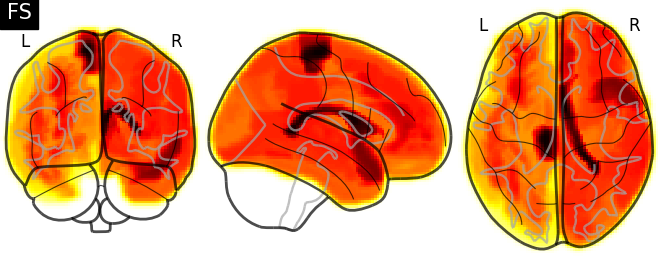
\includegraphics[width=0.42\textwidth]{images/biomarker-identification/fs.png}
    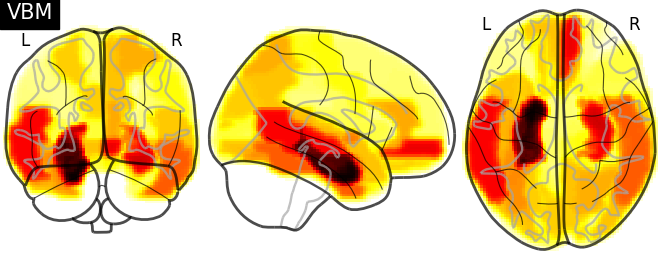
\includegraphics[width=0.42\textwidth]{images/biomarker-identification/vbm.png}
    \caption{Importance distribution over the brain regions. The darker color indicates the greater importance. The top five most important regions identified are {\bf FS:} Right Lateral Ventricle, Left Para-Hippocampal, Left Amygdala, Left Cerebral White Matter, Left Hippocampus, and {\bf VBM:} Left Para-Hippocampal, Left Amygdala, Left Hippocampus, Right Hippocampus, Right Amygdala.}
    \label{fig: brain map}
\end{figure}
\begin{figure}
    \centering
    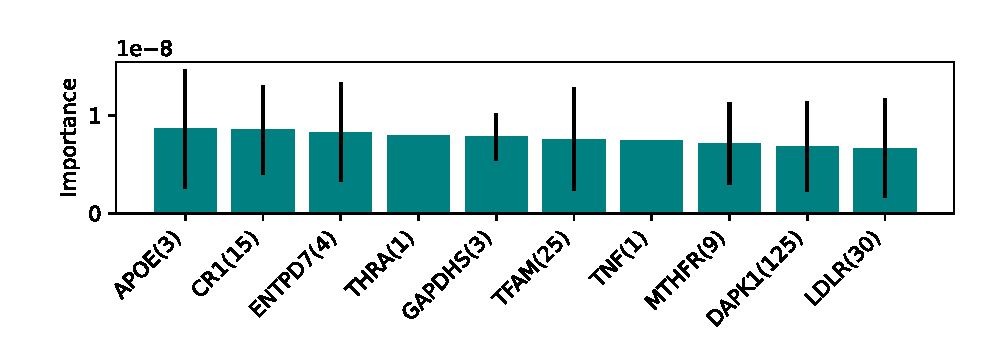
\includegraphics[width=0.85\textwidth]{images/biomarker-identification/alzgene-same-color.eps}
    \caption{Importance of each AlzGene group. The standard deviation and number of SNPs in each group is denoted by the line and the number next to the group name}\label{fig: AlzGene}
\end{figure}
% [Because of the dramatic increase in the prevalence of AD, the identification of effective biomarkers for the early diagnosis and treatment of AD in individuals at high risk to develop the disease is crucial.]
It is vital to identify AD relevant biomarkers for early detection and the treatment of people at high risk of developing AD. Despite the promising performance of deep neural networks, their predictions are notoriously difficult to interpret. To identify which biomarkers largely affect the predictions, we add the perturbation to the input data and observe the changes in prediction. The details of this identification method is described in supplementary. In Fig~\ref{fig: brain map} and Fig~\ref{fig: AlzGene}, we plot the importance distribution over the brain regions and AlzGene groups of SNPs. The AlzGene groups of SNPs have been constructed by the multiple genome-wide association studies listed on the website (\url{http://www.alzgene.org/}). From our model SAE, ventricular~\cite{carmichael2007ventricular}, hippocampus~\cite{mu2011adult}, and amygdala~\cite{poulin2011amygdala} are identified as important brain regions, and apolipoprotein E~\cite{kim2009role} and complement receptor 1~\cite{lambert2009genome} are identified as important AlzGene groups. The identified biomarkers have been shown in the literature to be related to AD, thus they provide substantial evidence that our approach can identify the biomarkers associated with AD.

% \begin{equation}\label{eq: SNPs identification}
% \begin{aligned}
%     &(\mathbf{x}_i^s)' = [x_{i, 1}^s, x_{i, 2}^s, \cdots, x_{i, m}^s + p_{i, m}, \cdots, x_{i, D_s}^s],\\
%     &\Delta\tilde{\mathbf{y}}_i = \| \psi_{pred}\bigl(\phi_{dynamic}(\mathbf{X}_i, \mathbf{M}_i, \mathbf{t}_i;\ \theta_{\phi}^d),\ \psi_{SNP}(\phi_{SNP}((\mathbf{x}_i^s)';\ \theta^s_{\phi});\ \theta^s_{\psi}),\ \mathbf{x}_i^b;\ \theta^p_{\psi}\bigr)\\
%     &- \psi_{pred}\bigl(\phi_{dynamic}(\mathbf{X}_i, \mathbf{M}_i, \mathbf{t}_i;\ \theta_{\phi}^d),\ \psi_{SNP}(\phi_{SNP}(\mathbf{x}_i^s;\ \theta^s_{\phi});\ \theta^s_{\psi}),\ \mathbf{x}_i^b;\ \theta^p_{\psi}\bigr)\|_1.
% \end{aligned}
% \end{equation}
% Finally, we plot top 15 most important features in Fig..
% \subsubsection{AD relevant imaging biomarkers}
% In Fig~\ref{fig: brain map}, we plot the importance distribution over the brain regions.
% % calculated by Eq.~\eqref{eq: neuroimaging identification}. 
% The identified regions have been shown in the literature to be related to AD. For example, the previous studies~\cite{carmichael2007ventricular} found that ventricular volume and its rate of change is related with vulnerability to cognitive decline and dementia. 
% % \cite{carmichael2007ventricular,jack2004comparison}
% They observe that the larger ventricles in healthy participants increase the probability to the progression of dementia-related disease in the future. The hippocampus is vulnerable to be damaged from AD~\cite{mu2011adult} and has been shown to affect long-term memory and spatial navigation in patients with AD. Finally, the amygdala region, also identified by our approach, is also severely affected by AD~\cite{poulin2011amygdala} and is associated with emotional response and decision-making.
% \subsubsection{AD relevant genetic biomarkers}
% We plot the importance distribution over the AlzGene groups of SNPs in Fig~\ref{fig: AlzGene}. The AlzGene groups of SNPs have been constructed by the multiple genome-wide association studies listed on the website (\url{http://www.alzgene.org/}). Apolipoprotein E (APOE) group is identified by our approach, and APOE genes involve in amyloid beta peptide (A$\beta$) aggregation and clearance~\cite{kim2009role}. The accumulation of A$\beta$ is commonly observed in the progress of AD~\cite{chen2017amyloid} and amyloid hypothesis suggests reasonable mechanism how the accumulation of A$\beta$ can result neuronal malfunction~\cite{hardy2002amyloid}. In addition, $\epsilon$4 allele of APOE gene increase risk factor for AD and decrease the age of AD onset~\cite{corder1993gene}. For complement receptor 1 (CR1) group, genome-wide analysis~\cite{lambert2009genome} reported CR1 association with late-onset AD. The subset of biomarkers identified in the FreeSurfer, VBM, and SNP modalities, provides substantial evidence that our approach can identify the biomarkers associated with AD.
% [Why multi-class classification? -> the different clinical actions are required for stage : AD, MCI, HC]
% even if very few samples are labeled.